% !TEX TS-program = pdflatex
% !TEX encoding = UTF-8 Unicode

% This is a simple template for a LaTeX document using the "article" class.
% See "book", "report", "letter" for other types of document.

\documentclass[11pt]{article} % use larger type; default would be 10pt

\usepackage[utf8]{inputenc} % set input encoding (not needed with XeLaTeX)

%%% Examples of Article customizations
% These packages are optional, depending whether you want the features they provide.
% See the LaTeX Companion or other references for full information.

%%% PAGE DIMENSIONS
\usepackage{geometry} % to change the page dimensions
\geometry{a4paper} % or letterpaper (US) or a5paper or....
% \geometry{margin=2in} % for example, change the margins to 2 inches all round
% \geometry{landscape} % set up the page for landscape
%   read geometry.pdf for detailed page layout information

\usepackage{graphicx} % support the \includegraphics command and options

% \usepackage[parfill]{parskip} % Activate to begin paragraphs with an empty line rather than an indent

%%% PACKAGES
\usepackage{booktabs} % for much better looking tables
\usepackage{array} % for better arrays (eg matrices) in maths
\usepackage{paralist} % very flexible & customisable lists (eg. enumerate/itemize, etc.)
\usepackage{verbatim} % adds environment for commenting out blocks of text & for better verbatim
\usepackage{subfig} % make it possible to include more than one captioned figure/table in a single float
% These packages are all incorporated in the memoir class to one degree or another...

%%% HEADERS & FOOTERS
\usepackage{fancyhdr} % This should be set AFTER setting up the page geometry
\pagestyle{fancy} % options: empty , plain , fancy
\renewcommand{\headrulewidth}{0pt} % customise the layout...
\lhead{}\chead{}\rhead{}
\lfoot{}\cfoot{\thepage}\rfoot{}

%%% SECTION TITLE APPEARANCE
\usepackage{sectsty}
\allsectionsfont{\sffamily\mdseries\upshape} % (See the fntguide.pdf for font help)
% (This matches ConTeXt defaults)

%%% ToC (table of contents) APPEARANCE
\usepackage[nottoc,notlof,notlot]{tocbibind} % Put the bibliography in the ToC
\usepackage[titles,subfigure]{tocloft} % Alter the style of the Table of Contents
\renewcommand{\cftsecfont}{\rmfamily\mdseries\upshape}
\renewcommand{\cftsecpagefont}{\rmfamily\mdseries\upshape} % No bold!

\renewcommand{\labelitemi}{$\bullet$}
\renewcommand{\labelitemii}{$\cdot$}
\renewcommand{\labelitemiii}{$\diamond$}
\renewcommand{\labelitemiv}{$\ast$}

%%% END Article customizations

%%% The "real" document content comes below...

\title{RASD}
\author{Giorgio Pea, Andrea Sessa}
%\date{} % Activate to display a given date or no date (if empty),
         % otherwise the current date is printed

\begin{document}
\maketitle
\newpage

\tableofcontents

\newpage

\section{Introduction}
  \subsection{Purpose}
    This document represent the Requirement Analysis and Specification Document
    (RASD). The main goal of this document is to completely describe the system
    in terms of functional and non-functional requirements, to show the constraints and the limit
    of the software and simulate the typical use cases that will occur after the
    development. This document is intended to all developers and programmers who
    have to implement the requirements, to system analysts who want to integrate
    other systems with this one, and could be used as a contractual basis between
    the customer and the developer.

  \subsection{Actual System}
    The whole project is built on the assumption that no preexistent system exists.
    Every feature and component of the new system has to be built without modifying
    or reusing parts of a previous system.

  \subsection{Scope of the project}
    The aim of this project is to develop MyTaxiService, a web/mobile application that makes easier and quicker taking taxies
    within the city's borders.
    Thanks to MyTaxiService, anyone can request or book a taxi and get realtime information
    about how long it will take to be picked up or about the taxi's current position and identification
    code.
    In addition to that, MyTaxiService provides an efficient way to allocate taxies by dividing the
    city in zones and using a queue based allocation system, in order to reduce the average
    waiting time and city's traffic.

  \subsection{Goals}
	\begin{enumerate}
	    \item Simplify and speed up the process of taking a taxi within the city's borders
		\begin{enumerate}
		      \item When a registered user has entered his taxi ride details and clicks or taps
		      the "REQUEST TAXI" button, MyTaxiService will find the first
		      available mtaxi that fits for the inserted ride details, and this mtaxi will
		      pick up the registered user as soon as possible
		
		      \item When a registered user has entered his booking details and clicks or taps
		        the "BOOK TAXI" button, MyTaxiService will book a mtaxi that fits for the
		        inserted booking details and for the indicated pick up time
		\end{enumerate}
	
	    \item Guarantee an efficient and fair management of taxi queues
	  	\begin{enumerate}
		      \item Guarantee a balanced distribution of mtaxies in the city, in order
		      to have them always available for different city zones
		
		      \item Guarantee short mtaxi availability times and short waiting times
		\end{enumerate}
	\end{enumerate}

  \subsection{Assumptions}
	\begin{enumerate}
	    \item MyTaxiService has been commissioned by the city's local government.
	
	    \item The local government provides each mtaxi with a device similar to a small navigator(MYT). This device is used
	      to: see and accept ride/booking requests, see zone change orders, report accidents; it has a built in gps module through which MyTaxiService can
	      track the position of the mtaxi on which is mounted
	
	    \item Mtaxies can only serve ride/booking requests forwarded by MyTaxiService(B)
	
	    \item Mtaxies operate only whithin the city's borders
	\end{enumerate}

  \subsection{Terms and definitions}
	\begin{description}
	      \item [User] \hfill \\A generic person not registered to MyTaxiService
	      \item [Passenger] \hfill \\ a registered user that has requested a mtaxi ride/booking
	      \item [Registered User] \hfill \\ A generic person that is registered to MyTaxiService
	      \item [Mtaxi] \hfill \\ a taxi that joined MyTaxiService
	      \item [MyTaxiService(B)] \hfill \\ The back end of MyTaxiService, that is to say, those software components
	        that manage the forwarding of ride/booking requests to mtaxi drivers, the search of available mtaxies compatible with the received ride/booking requests, the distribution
	        of mtaxies in the different city's zones and other internal tasks not exposed to users or mtaxi drivers
	      \item[Ride] \hfill \\ A movement of people, through a taxi cab, from one location to another
	      \item [Ride request] \hfill \\ An electronic message sent by a registered user
	        to MyTaxiService(B). This electronic message refers to the case in which the registered user wants to be picked up as soon as possible by a mtaxi
	      \item[Booking request]\hfill \\ An electronic message sent by a registered user
	         to MyTaxiService(B). This electronic message refers to the case in which the registered user wants to be picked up by a mtaxi at a specific date and time
	      \item[Mtaxi booking, booking a ride] \hfill\\If a registered user wants to be picked up by a mtaxi at specific date and time, he books a ride or a mtaxi
	      \item [MYT] \hfill \\The device the local government provides to taxi drivers that have registered to MyTaxiService. This
	      device integrates a client for MyTaxiService that is used by the mtaxi driver to see ride/booking requests and zone change orders, accept
	      these requests and report accidents
	      \item [A mtaxi is available] \hfill \\ A mtaxi has finished serving a passenger and is ready for a new ride
	      \item [A mtaxi is unavailable]\hfill \\ A mtaxi is considered unavailable if and only if or is serving a passenger or has reported an accident or
	      is stuck in the traffic(and this has been detected by MyTaxiService(B))
	      \item [Zone] \hfill \\An area of the city about $2km^2$ wide
	      \item [Credentials] \hfill \\ A combination of username and password, used by a registered user to access the MyTaxiService application
	      \item [Queue] \hfill \\ A data structure managed with a FIFO policy.
	      \item [Ride/booking request acceptance] \hfill \\ A mtaxi driver has accepted a ride/booking request if he has left in order to pick up the passenger
	      associated with the request
	      \item [The city] \hfill \\The city that is served by MyTaxyService and its taxies
	\end{description}

    \subsection{Acronyms}
      \begin{itemize}
		\item \textbf{RASD:} Requirements Analysis and Specification Document
      		\item \textbf{FIFO:} First In First Out
      \end{itemize}

    \subsection{Reference Documents}
	\begin{itemize}
	      \item Specification Document: MyTaxiService-AA2015-2016.pdf
	      \item IEEE Std 830-1998 IEEE Recommended Practice for Software Requirements Specifications.
	      \item  IEEE Std 1016 tm -2009 Standard for Information Tecnology-System Design-Software Design Descriptions.
	\end{itemize}

      \subsection{Main Actors}
	See Terms and Definitions section
	\begin{itemize}
	        \item User
	        \item Registered User
	        \item Mtaxi driver
	        \item Taxi driver
	        \item MyTaxiService(B)
	\end{itemize}

\section{Requirements Specification}
    \subsection{Functional requirements}

      The following table shows the only functionalities of MyTaxiService accessible by
      the different actors:
      \begin{enumerate}
	      \item USER
		\begin{enumerate}
		      \item User registration
		\end{enumerate}
	
	      \item REGISTERED USER
		\begin{enumerate}
		      \item Login
		      \item Remember me (see below for details)
		\end{enumerate}
	
	      \item LOGGED REGISTERED USER
		\begin{enumerate}
		      \item Logout
		      \item Request a ride
		      \item Book a ride
		      \item View the status of a ride (requested or booked)
		      \item Undo a ride booking (If possible)
		\end{enumerate}
	
	
	      \item TAXI DRIVER
		\begin{enumerate}
		      \item Taxi driver registration
		\end{enumerate}
	
	      \item MTAXI DRIVER
		\begin{enumerate}
		      \item Accept a ride request/booking
		      \item Complete a ride
		      \item View the details of ride request/booking
		      \item Report an accident
		\end{enumerate}
	
	      \item A user can register to MyTaxiService only and only once
	      \item MyTaxiService has to be able to remember logged sessions so that when a registered user
	      opens next time the MyTaxiService app or website, he has not to log in again (Remember me functionality)
	      \item MyTaxiService has to implement a user registration process that requires the user to insert: name, lastname,
	      email, password
	      \item MyTaxiService has to implement a taxi driver registration process that requires the user to insert: name, lastname,
	      email, password
	      \item During the user registration process, MyTaxiService has to be able to check the formal validity of the
	      data inserted by the user
	      \item MyTaxiService has to only accept user registrations with mail addresses not already used by other
	      registered users
	      \item MyTaxiService has to only accept registrations whose data formal validity has been
	      check successfully
	      \item Logged registered users can undo a reservation only 10 minutes before the inserted
	      picking up time
	      \item MyTaxiService has to allow multiple mtaxi bookings by the same logged registered user
	      \item MyTaxiService has not to allow multiple ride requests by the same logged registered user
	      (a registered user can't make a new ride request until his last requested ride has been completed)
	      \item MyTaxiService can accept only ride requests that specify a starting location, an ending location
	      and a number of passengers
	      \item MyTaxiService has to be able to access a list of every valid city's location
	      \item MyTaxiService has to be able to access realtime data about the city's traffic
	      \item MyTaxiService has to force a logged registered user to choose as starting/ending locations of a ride only valid city's locations
	      \item MyTaxiService has to force a logged registered user to chose among a list of only valid city's locations
	      \item MyTaxiService has to force a logged registered user not choose the same location as starting and ending location of a ride
	      \item MyTaxiService(B) has to be able to retrieve the position of each mtaxies using the gps system of their MYT devices
	      \item MyTaxiService(B) has to be able to logically divide the city in zones and associate sets of gps
	      coordinates to these zones
	      \item MyTaxiService(B) has to be able to map a gps coordinate with a valid city's location
	      \item MyTaxiService(B) has to be able, using the mtaxies' gps data and the city's public data, to understand the
	      city's traffic situation zone by zone (High traffic, normal traffic, low traffic)
	      \item MyTaxiService(B) has to be able, using the mtaxies' gps coordinates, to analyze their
	      distribution among the different city's zones and understand if there's the need to change this
	      distribution in relation to the average number of ride/booking requests per city's zone.
	      \item MyTaxiService(B) has to be able to send change zone order to mtaxies
	      \item MyTaxiService(B) has to be able, using mtaxies' gps coordinates, to analyze the mtaxies'
	      distribution among the different city's zone and build queues of available mtaxies for each zone
	      \item MyTaxiDriver(B) has to manage the forwarding of ride/booking requests using the queue based system discussed above:
	      a ride/booking request is forwarded to the first mtaxi in the queue that corresponds to the city's zone of the requested ride's
	      starting location
	      \item MyTaxiService(B) has to be able to manage a situation in which a mtaxi does not accept a ride/booking request within a fixed time.
	      In this situation MyTaxiService has to find a new mtaxi to forward the request
	      \item MyTaxiService app and website must have the same functionalities
	      \item MyTaxiService(B) has to have access to the characteristics of each mtaxies (number of passengers, unique code)
	      \item MyTaxiService(B) has to have access to the mtaxi drivers' work timetable, in order to know when a mtaxi should start
	      serving passengers, should take a lunch break or should finish all activities
	      \item MyTaxiService has to consider unavailable only mtaxies that or are serving a ride/booking request or have reported an accident or
	      are taking a break according to the work timetable, no other exceptions are allowed
	      \item MyTaxiService has to offer to mtaxi drivers the possibility of reporting an accident and therefore be considered unavailable
	\end{enumerate}

    \subsection{Non functional requirements}
	\begin{enumerate}
	      \item MyTaxiService has to guarantee that a mtaxi arrives at the start location of a ride within 10 minutes
	      \item A mtaxi driver has to accept a ride/booking request within 2 minutes
	      \item After a failure MyTaxiService has to be restarted within 1 hour
	      \item MyTaxiService must be available 24h/7d
	      \item Registered users have to be able to use properly all MyTaxiService's functionalities after a training time of at most 15 mins
	      \item All MyTaxiService's functionalities have to be reachable by a registered user with at most 3 clicks/taps from the after login screen
	      of the web/mobile app
	\end{enumerate}

      \subsubsection{Security}
        Among non functional requirements particular attention must be devoted to security aspects.
        During the login MyTaxiService has to prevent malicious users from phishing sensible data(password, username etc) by adopting suitable
        protection mechanism(password encryption, encrypted communication protocols etc).
        From the server side MyTaxiService must guarantee that data access from remotes users is controlled and filtered such that
        no unauthorized access(SQL injection, MITM attack, etc) to sensible data is permitted.
\newpage
      \subsubsection{Interfaces Requirements}
       In this section is shown a series of mock up that specify a set of requirements over the user interface.\newline
       Each mock up is valid both for the web site and mobile application version of MyTaxiService\newline 
        \newline
        This mock up shows the user login page\newline
       \newline
        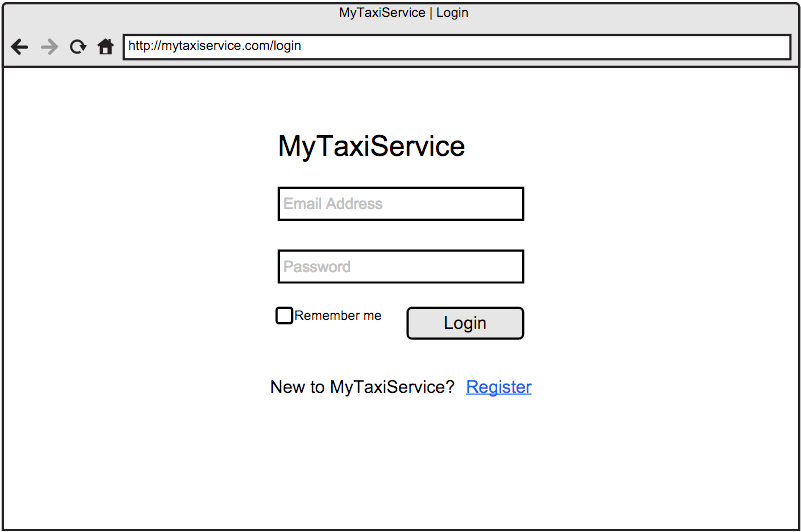
\includegraphics[scale=0.52]{loginInt.png}\newline
        \newpage
        \noindent
        This  mock up shows the user registration page\newline
	\newline
        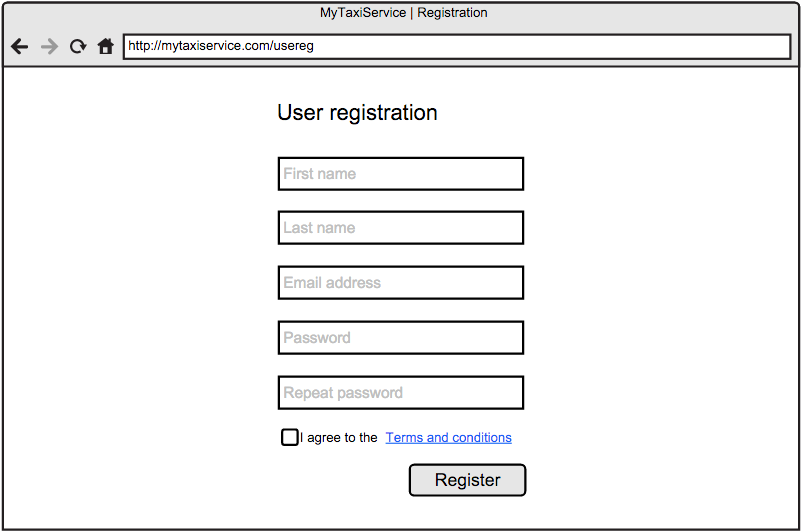
\includegraphics[scale=0.52]{userRegInt.png}\newline
        \newpage
        \noindent
        This mock up shows the user ride request page\newline
        \newline
        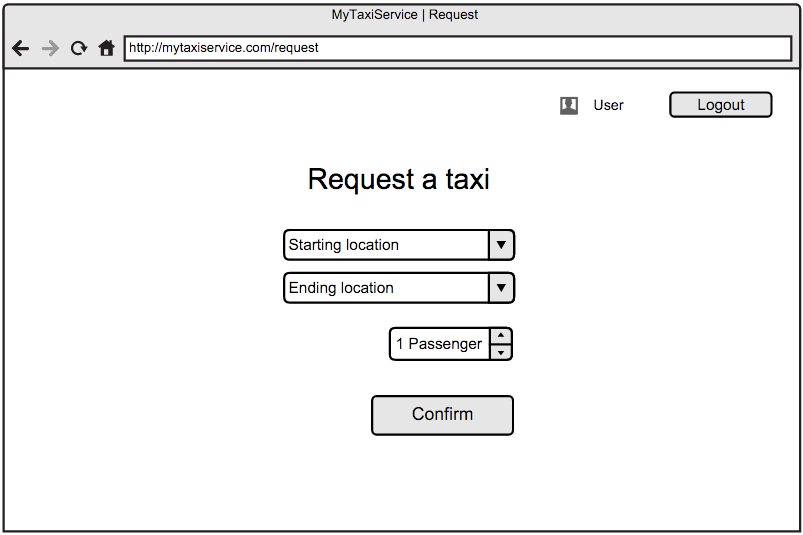
\includegraphics[scale=0.52]{taxiReqInt.png}\newline
        \newpage
        \noindent
        This mock up shows the user ride booking page\newline
       \newline
        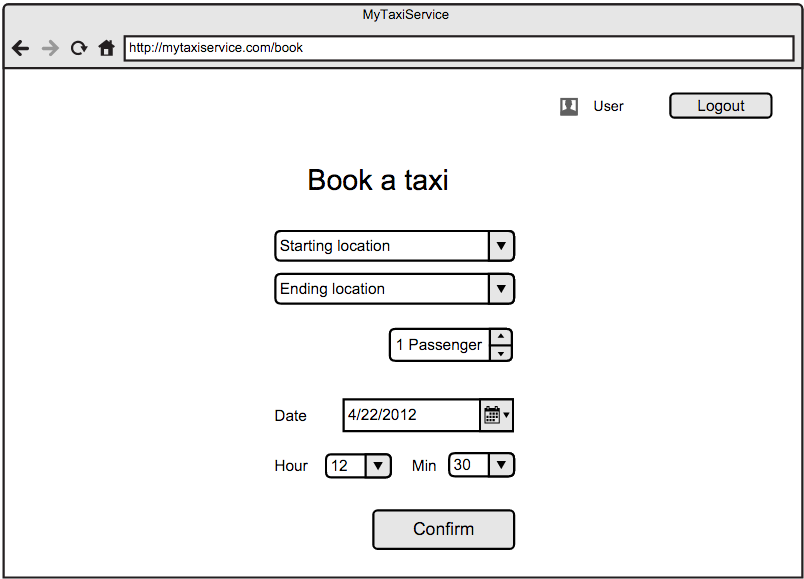
\includegraphics[scale=0.52]{taxiBookInt.png}\newline
        \newpage
        \noindent
        This mock up shows the empty booking/ride request view page\newline
        \newline
        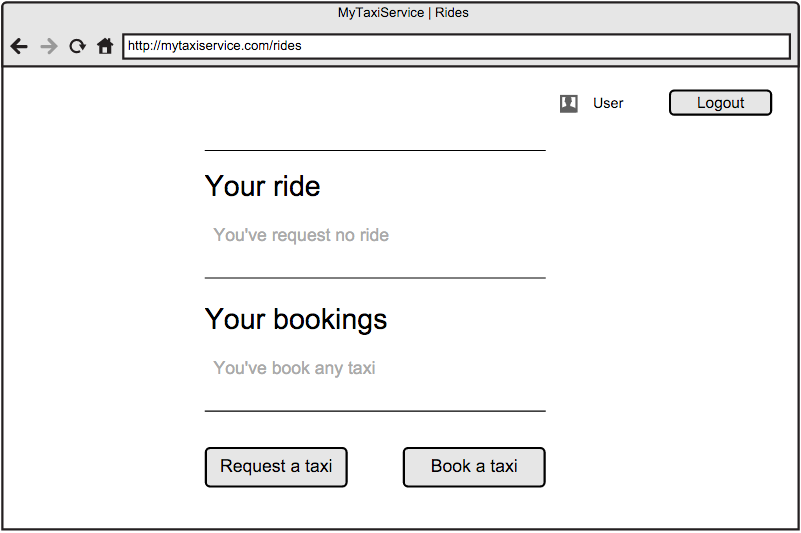
\includegraphics[scale=0.52]{viewEmptyInt.png}\newline
        \newpage
        \noindent
        This mock up shows the booking/ride request view page when the user has requested a ride \newline
        \newline
        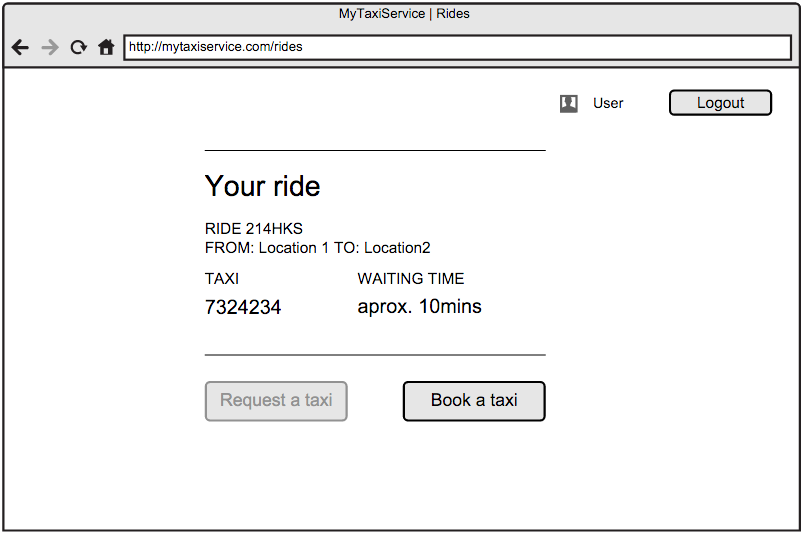
\includegraphics[scale=0.52]{viewReqInt.png}\newline
        \newpage
        \noindent
        This mock up shows the booking/ride request view page when the user has booked and requested a ride\newline
        \newline
        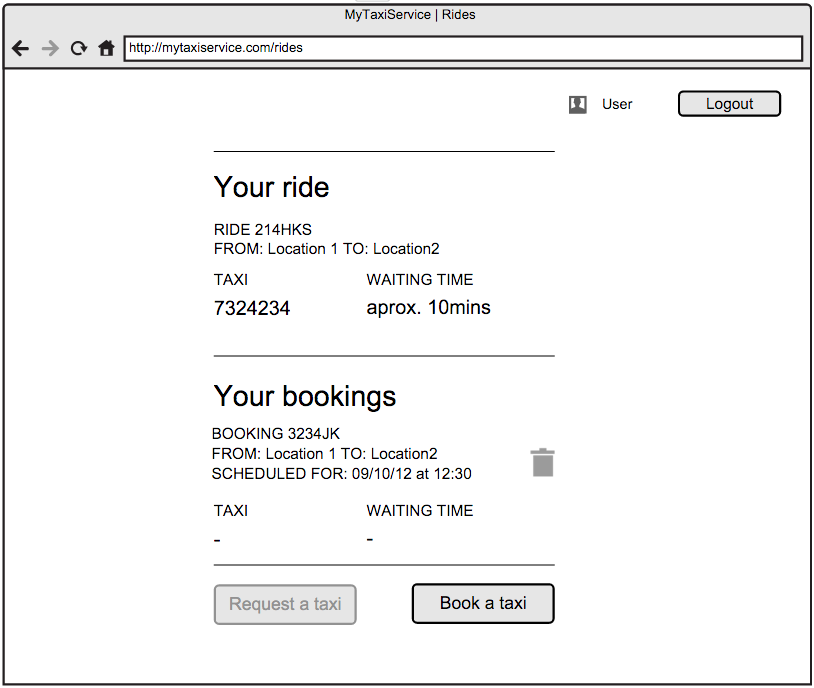
\includegraphics[scale=0.52]{viewReqBookPage.png}\newline
        \newpage
        \noindent
        This mock up shows the deletion of a booking request by a registered user\newline
        \newline
        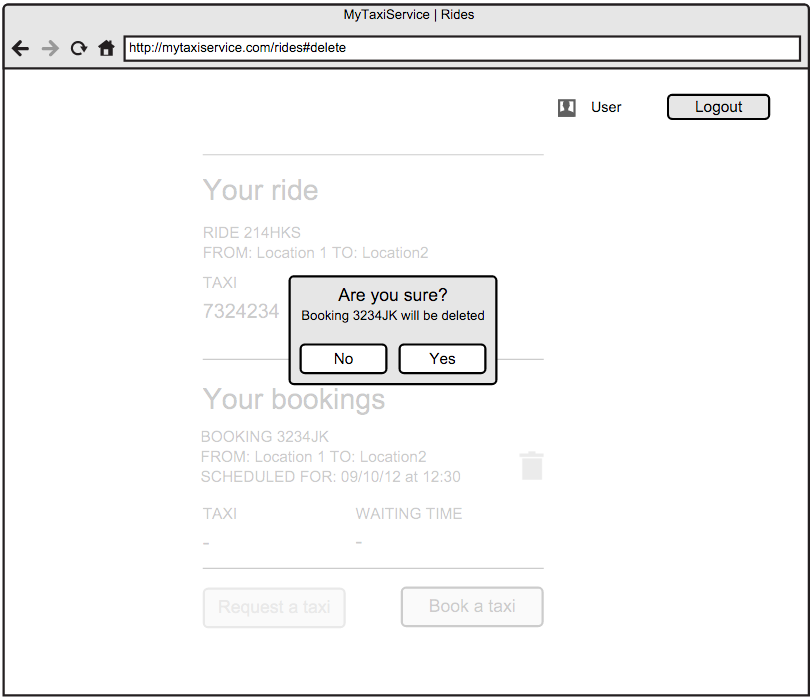
\includegraphics[scale=0.52]{deleteBookInt.png}\newline
        \newline
        

    \subsection{Constraints}
	\begin{enumerate}
	      \item MyTaxiService rquires Android 2.0 (or later) or IOS 6.0 (or later)
	\end{enumerate}

    \subsection {Domain Properties}
	\begin{enumerate}
	      \item Traffic information are reliable
	      \item GPS data are reliable
	      \item If a registered user request a RideRequest then then he will be present at the starting point when the taxi arrives
	\end{enumerate}

\section {Scenarios, Use Case and UML diagrams}

    \subsection{Scenarios}
	\begin{enumerate}
	    \item Bob is a product manager with a very busy schedule. At 11.00 he has a meeting
	       with a group of clients to discuss about the features of a new product.
	       This meeting is located in a another part of the city.
	       For his shifts Bob usually takes taxies, and, in order to speed up this process, he
	       started using MyTaxiService.
	       It's 10:30 and Bob decides to take a taxi via MyTaxiService. He opens the app,
	       the app remembers his credentials and logs him in.
	       Bob inserts the address of the meeting and of his current location, choses one passenger and taps
	       the "REQUEST TAXI" button. MyTaxiService then alerts him that is finding a mtaxi.
	       Near Bob's location, a mtaxi has finished serving a passenger, so MyTaxiService(B) signals to it
	       Bob's request. Charlene, the driver of the mtaxi, despite the fact that it's still work time, she wants to take a coffee
	       and so ignores the request. After 5 mins MyTaxiService(B) tries to find a new mtaxi
	       for Bob: Albert's mtaxi is available and MyTaxiService(B) forwards Bob's request to it.
	       Albert receives the request and alerts MyTaxiService(B) that he's going to take care of the ride.
	       MyTaxiService alerts Bob that his taxi will arrive in 3 mins.
	       The Taxi arrives, and in 10 mins Bob reaches the meeting place. MyTaxiService(B)
	       signals the behavior of Charlene to her supervisors, and, after a few weeks, Charlene receives a warning and a fine of 200 euro
	
	    \item It's Friday, 10 a.m, Paris, Ann, a young american tourist, has to take a flight at 12 a.m to return to New York City.
	        Ann has carefully planned the return trip, infact
	       yesterday she made a taxi booking via MyTaxiService web site for 9:45 a.m , but the mtaxi has not arrived yet.
	       So she take her smartphone opens the MyTaxiService application, enters her credentials and after a successful login
	       she discovers that her mtaxi is stuck in a terrible traffic jam and that MyTaxiService is trying to find a new mtaxi.
	       "I'll miss my flight!" she thinks, and starts to wait with the heart full of hope
	
	    \item Dave, an experienced taxi driver of the city, has received, through MyTaxiService, a request for a ride
	       from a passenger. "It's not too much far from where i am now", he thinks, "It'll be easy", and notifies
	       MyTaxiService that he'll take care of the request. He starts driving toward the passenger's position, but suddenly
	       , while he's crossing a very busy crossroad,
	       a reckless driver coming from the left crosses at high speed the crossroad and hits with violence
	       Dave's taxi cab. Luckily nobody gets hurt, but Dave's taxi cabe has been seriously damaged.
	       Dave cannot fulfill the passenger's request so he takes his smartphone, opens the MyTaxiService app,
	       and taps the "REPORT ACCIDENT" button, he accesses a screen where he inserts the accident details and taps the "SUBMIT" button.
	       MyTaxiService(B) receives the Dave's report and after some computations selects and notifies another driver to fulfill the passenger request.
	
	    \item Ann, a young female student from Texas, is visiting Italy with his boyfriend Bob.
	      It's Friday morning, they are walking on the streets of Milan and they're thinking
	      about visiting the Expo on Saturday. Ann proposes to use a taxi to reach Expo's location and
	      Bob agrees. Ann is a very cautious person so she thinks it's better to book a taxi, for this
	      reason she searches on Google "taxi milano book" and discovers MyTaxiService.
	      She downloads the app on her Iphone; she opens the app, which displays a login screen with
	      a registration button, and taps that button being so redirected to a registration screen; she inserts
	      her mail address, choses and confirm a password, accepts the legal
	      terms of the app and taps the confirm button; after that Ann is ready to use the app.
	      In order to book a taxi for Saturday for the Expo, Ann accesses the booking section of the app,
	      taps the "ADD BOOKING" button and in the add booking screen inserts the Expo's location by selecting the right item in a dropdown menu, inserts the time and location of the picking
	      , choses two passengers and taps the big "BOOK TAXI" button, MyTaxiService responds by alerting Ann that her booking
	      has been processed successfully. Ann is happy about the fact that everything has proceeded without problems.
	      Bob instead is not so happy because he thinks that the Milan's transportation system is perfect
	      to reach Expo and its far way cheaper than taking a taxi. Bob and Ann have a brief discussion
	      about this and, at the end, Ann agrees with Bob. Given that, Ann tries to undo the booking:
	      she opens the app, she logs in, she accesses the booking section and there she sees her booking for Saturday, she taps
	      the bin icon to delete the booking, she confirms her intention to do that and everything is done.
	
	    \item It's Thursday, 14:00 and George, a young mtaxi driver, is driving in the city's center.
	       He noticed many of his colleagues waiting for requests in their cabs.
	       Meanwhile MyTaxiService(B), by making some analysis on the mtaxies' GPS data, realizes that there are too many mtaxies
	       in the city's center in relation with the number of ride requests for that zone. The system also indentifies
	       some zones of the city where the concentration of taxies is too low. According to a policy based on some statistical data
	       MyTaxiService(B) decides to move 10 mtaxies, including the George's one, from the city's center to the city's zones mentioned above.
	       As a consequence of that, George receives by MyTaxiService a notification that alerts him to move to zone C (one of the city's zones
	       with low concentration of mtaxies). George start driving towards zone C and continues his work.
	\end{enumerate}

    \subsection{Use cases of the application}

      1. A registered user makes a ride request
        [Actors]: A registered user, MyTaxiService(B)
        [Pre-cons]: The registered user has logged into MyTaxiService.
        [Post-cons]: MyTaxiService(B) receives the ride request and tries to find an available taxi to fulfill it.
        [Entry Cnd]: A registered user wants to be picked up by a mtaxi as soon as possible in a given place.
        [Exit Cnd]: The registered user is acknowledged that MyTaxiService(B) has received successfully the ride
        request
        [Exceptions]:
          - Connection lost(for the mobile app): the registered user is immediately notified of the event and
          asked to try again later
        [Flow of events]:
          - The registered user taps/clicks the "REQUEST TAXI" button
          - The registered user is redirected to a screen dedicated to the insertion
          of the requested ride's details
          - The registered user fills out a form for the ride request inserting the ride's starting and ending location
          (chosen from a list of every valid city's location) and the number of passengers
          - The registered user submits to MyTaxiService(B) the form by clicking/tapping the "CONFIRM REQUEST" button

      --------------------------------------------------------------------------------

      2. A registered user makes a booking request
         [Actors]: A registered user, MyTaxiService(B)
         [Pre-cons]: The registered user has logged into MyTaxiService.
         [Post-cons]: MyTaxiService(B) receives the booking request and registers it; 10 mins before
         the chosen picking up time, MyTaxiService(B) will try to find an available taxi to fullfill the request
         [Entry Cnd]: A registered user wants to book a mtaxi in order to be picked up at a specific date and time
         [Exit Cnd]: The registered user is acknowledged that MyTaxiService(B) has received successfully the ride
         request
         [Exceptions]:
           - Connection lost(for the mobile app): the registered user is immediately notified of the event and
           asked to try again later
         [Flow of events]:
           - The registered user taps/clicks the "BOOK TAXI" button on the home screen of the app/website
           - The registered user is redirected to a screen dedicated to the insertion
           of the requested booking details
           - The registered user fills out a form for the booking request, inserting the ride's starting and ending location,
           the number of passengers, the date and the time for which be picked up.
           - The registered user submits to MyTaxiService(B) the form by clicking/tapping the "CONFIRM BOOKING" button

      --------------------------------------------------------------------------------

      3. MyTaxiService(B) forwards a received ride request to a mtaxi driver
        [Actors]: A mtaxi driver, MyTaxiService(B)
        [Pre-cons]: The mtaxi driver has informed MyTaxiService(B) that he has finished serving a passenger and so is
        ready for a new ride
        [Post-cons]: The mtaxi driver knows that a registered user has requested a ride with the specified
        details and is ready to fulfill it
        [Entry Cnd]: MyTaxService(B) has received a ride request from a logged registered user
        [Exit Cnd]: MyTaxiService(B) is acknowledged that the mtaxi driver has received successfully the ride request
        [Exceptions]:
          - No mtaxi is available for the city's zone relative to the ride request: MyTaxiService(B) tries
          to find a mtaxi that fits the ride request details(in terms of number of passengers) and that is located in the city's zones adjacent
          to the one above mentioned
          - No mtaxi available: MyTaxiService(B) notifies the registered user who made the request, that
          no mtaxi is available and that he should try again later
        [Flow of Events]:
          - MyTaxiService(B) extracts the city zone relative to the starting location of the ride request
          - MyTaxiService(B) selects a mtaxi that suits the ride requests details (in terms of number of passengers) from the queue of available mtaxies
            for the city zone above mentioned
          - MyTaxiService(B) checks if the traffic conditions in the zone where the selected mtaxi is located are acceptable
          (they allow the mtaxi to reach the registered user to pick up within a fixed time)
          - MyTaxiService(B) forwards the ride request to the driver of the selected mtaxi


      -------------------------------------------------------------------------------

      4. A mtaxi driver informs MyTaxiService(B) that he has finished serving a passenger
        [Actors]: A mtaxi driver, MyTaxiService(B)
        [Pre-cons]: The mtaxi current location is the ending location of his last ride
        [Post-cons]: MyTaxiService(B) considers the mtaxi available
        [Entry Cnd]: The mtaxi driver has finished serving a passenger
        [Exit Cnd]: The mtaxi driver is acknowledged that MyTaxiService(B) has received successfully his
        notification
        [Exceptions]:
          - Connection Lost: the mtaxi driver is immediately notified of the event and is asked to try again
          later
        [Flow of Events]:
          - The mtaxi driver taps the "END RIDE" button on the screen of his MYT and so notifies MyTaxiService(B) that
          he has ended serving a passenger and is now available for other ride/booking requests


      --------------------------------------------------------------------------------

      5. A mtaxi driver manages a ride request from MyTaxiService(B)
        [Actors]: A mtaxi driver, MyTaxiService(B)
        [Pre cons]: The mtaxi has to be available
        [Post cons]: The mtaxi driver has started driving to the starting location of the requested ride
        [Entry Cnd]: MyTaxiService(B) has forwarded successfully a ride request to the mtaxi driver
        [Exit Cnd]: The mtaxi driver is acknowledged that MyTaxiService(B) has received successfully his notification
        of ride acceptance.
        [Exceptions]:
          - If MyTaxiService(B) does not receive the acceptance of the ride request by the mtaxi driver
          within 5 mins, it selects another mtaxi to fullfil the request, and signals to the supervisors
          of the mtaxi driver in discussion his behavior
        [Flow of Events]:
          - The mtaxi driver taps the "ACCEPT REQUEST" button on the screen of his MYT, and so notifies MyTaxiService(B)
          that he's going to take immediately care of the request


      --------------------------------------------------------------------------------

      6. A registered user logs into MyTaxiService
        [Actors]: A registered user, MyTaxiService(B)
        [Pre Cnd]: The registered user is not logged into MyTaxiService. The registered
        user has access to MyTaxiService app or website
        [Post Cnd]: The registered user has access to all the functionalities of
        MyTaxiService reserved to registered users(see functional reqs)
        [Entry Cnd]: The registered user wants to access the functionalities offered by MyTaxiService
        [Exit Cnd]:  The registered user is acknowledged that MyTaxiService(B) has recognized as valid the inserted
        credentials. MyTaxiService(B) will grant the registered user the access to all the functionalities
        reserved to registered users(see functional reqs)
        [Exceptions]:
          - Connection Lost: the registered user is immediately notified of the event and the entire process
          has to be redone
          - Wrong Credentials(credentials that do no match any registered used): the registered user is asked to insert his credentials again
        [Flow of Events]:
          - The registered user opens the MyTaxiService app or access the MyTaxiService website, and a login
          screen is shown, along with the option to register to the service and to rembember the login
          - The registered user inserts his credentials in the relative fields
          - The registered user clicks/taps the "LOGIN" button

      --------------------------------------------------------------------------------

      7. A registered user logs out from MyTaxiService
        [Actors]: A registered user, MyTaxiService(B)
        [Pre cons]: The registered user is logged into MyTaxiService
        [Post cons]: The registered user has no access to MyTaxiService functionalities
        until a new login
        [Entry Cnd]: The registered user wants to logout from MyTaxiService
        [Exit Cnd]: The registered user is acknowledged that MyTaxiService(B) has logged him out from
        the service
        [Exceptions]:
          - Connection Lost: the registered user is immediately notified of the event and the entire process
          has to be redone
        [Flow of Events]:
          - The registered user taps/clicks the "LOGOUT" button on a screen of the app/website
          (every screen of the app/website has the "LOGOUT" button)

      --------------------------------------------------------------------------------

      8. A User wants to register to MyTaxiService
        [Actors]: A user, myTaxiService(B)
        [Pre cons]: The user has access to the MyTaxiService app or website
        [Post cons]: The user becomes a registered user
        [Entry Cnd]: The user wants to register to MyTaxiService in order
        to access its functionalities
        [Exit Cnd]: The user is acknowledged that MyTaxiService(B) has registered him
        [Exceptions]:
          - Connection Lost: the user is immediately notified of the event and the entire process
          has to be redone
          - Invalid data(non correctly formatted data or a email already
          user by another registered user): the user is immediately notified and forced to insert valid data
        [Flow of Events]:
          - The user opens the MyTaxiService app or access the MyTaxiService website, and a login
            screen is shown, along with the option to register to the service
          - The user taps/click the "REGISTER TO THE SERVICE" button
          - The user is redirected to a screen with a form to be filled out with Name, Surname, email a password.
          - The user fills the form
          - The user press the "CONFIRM BUTTON" and so submits the form to MyTaxiService(B)

      --------------------------------------------------------------------------------

      9. A registered user undoes a mtaxi booking
        [Actors]: A registered user, MyTaxiService(B)
        [Pre cons]: The registered user is logged into MyTaxiService. The registered user
        has made a successful booking request. The mtaxi booking the registered user wants to undo
        specifies a pickup time so that (pickuptime - currentime) > 10 mins
        [Post cons]: The scheduled booking is no more
        [Entry Cnd]: The registered user wants to undo a mtaxi booking
        [Exit Cnd]: MyTaxiService(B) acknowledges the registered user that the scheduled booking
        has been deleted
        [Exceptions]:
          - Connection Lost: the registered user is immediatly notified of the event and the entire process
          has to be redone
        [Flow of Events]:
          - The registered user accesses the MyTaxiService app/website area where he can see the list of his bookings
          - The registered user taps/click the recycle bin icon located in the row that corresponds to the mtaxi booking
          he wants to undo
          - The registered user confirm his choice by clicking/tapping the "CONFIRM" button on
          the popup that has just apparead

      --------------------------------------------------------------------------------

      10. A mtaxi driver receives a zone change order
        [Actors]: A mtaxi driver, MyTaxiService(B)
        [Pre cons]: The mtaxi is available
        [Post cons]: The distribution of mtaxies in the city's zones is more balanced
        with respect to the average number of ride requests per zone
        [Entry Cnd]: MyTaxiService(B) has detected that some city's zones have too much mtaxies assigned
        and some others not, all with respect to average number of ride requests per zone. MyTaxiService
        has assigned the mtaxi in discussion to another city's zone
        [Exit Cnd]: MyTaxiService(B) is acknowledged by the mtaxi driver that he has received successfully
        the zone change order
        [Exceptions]:
          - Connection Lost: the mtaxi driver is immediately notified of the event and the entire process has to be redone
        [Flow of Events]:
          - MyTaxiService(B) forwards to the mtaxi a change zone order, since the mtaxi has been assigned to another city's zone in order to guarantee
          a more balanced distribution of mtaxies among all the city's zones
          - The mtaxi driver receives the order

      --------------------------------------------------------------------------------

      11. A mtaxi driver reports an accident
        [Actors]: A mtaxi driver, MyTaxiService(B)
        [Pre cons]: The mtaxi driver has access to and can use MYT. MYT has not been damaged and so
        is fully functional
        [Post cons]: MyTaxiService(B) considers the mtaxi not available and stores the data
        relative to the accident for statical uses
        [Entry Cnd]: A mtaxi driver had an accident and wants to report it(has to report it)
        [Exit Cnd]: MyTaxiService(B) acknowledges the driver about the fact that it has received
        successfully the accident report
        [Exceptions]:
          - Connection Lost: the mtaxi driver is immediately notified of the event and the entire process has to be redone
        [Flow of Events]:
          - The mtaxi driver taps the "REPORT ACCIDENT" button on the screen of his MYT

      --------------------------------------------------------------------------------

      12. mtaxi registration
        [Actors]: A taxi driver, MyTaxiService(B)
        [Pre cons]: The taxi driver is not yet registered to MyTaxiService
        [Post cons]: The taxi driver becomes a mtaxi driver.
        [Entry Cnd]: A taxi driver wants to register to MyTaxiService
        [Exit Cnd]: The taxi driver is acknowledged that MyTaxiService(B) has registered him. MyTaxiService(B)
        assigns to the taxi a unique identification number
        [Exceptions]:
          - Connection Lost: the taxi driver is immediately notified of the event
          - The taxi is not registered as a city's taxi: the taxi driver is immediately notified
          and forced to change personal and taxi cab information inserted
        [Flow of Events]:
          - The taxi driver access the MyTaxiService website, and a login
            screen is shown, along with the option to register to the service
          - The taxi driver click the "REGISTER TO THE SERVICE AS NEW DRIVER" button
          - The taxi driver is redirected to a screen with a form to be filled out with personal information (name, surname, address, SSN) and
           taxi cab information(brand and model, license plate number)
          - The taxi driver fills the form
          - The taxi driver press the "CONFIRM BUTTON" and so submits the form to MyTaxiService(B)



\end{document}
